% !TEX program = pdflatex

\documentclass[journal,twoside]{IEEEtran}
\usepackage[T1]{fontenc}
\usepackage{amssymb,amsmath,amsfonts,amsthm}
\usepackage{graphicx}
\ifCLASSOPTIONcompsoc
  \usepackage[caption=false, font=normalsize, labelfont=sf, textfont=sf]{subfig}
\else
  \usepackage[caption=false, font=footnotesize]{subfig}
\fi
\interdisplaylinepenalty=2500
%\usepackage[cmintegrals]{newtxmath}
\usepackage{bm}
\usepackage[noadjust]{cite}
\usepackage{footnote}
\usepackage{xcolor}
\makesavenoteenv{tabular}
\usepackage{algorithm}
\usepackage{algpseudocode}
\usepackage{pgfplots}
\usepackage{threeparttable}
\usepackage{booktabs}
\usepackage{colortbl}
\usepackage{scalerel}
\usepackage{wrapfig}
\usepackage{listings}

\usepackage{tikz}
\usepackage{adjustbox}
\usetikzlibrary{svg.path}
\pgfplotsset{compat=newest}
\PassOptionsToPackage{hyphens}{url}\usepackage[hidelinks]{hyperref}
\hypersetup{breaklinks=true}

\newtheorem{proposition}{Proposition}

\definecolor{dkgreen}{rgb}{0,0.6,0}
\definecolor{gray}{rgb}{0.5,0.5,0.5}
\definecolor{mauve}{rgb}{0.58,0,0.82}
\lstset{
  numbers=none,  
  frame=tb,
  aboveskip=3mm,
  belowskip=3mm,
  showstringspaces=false,
  columns=fixed,
  framerule=1pt,
  rulecolor=\color{gray!35},
  backgroundcolor=\color{gray!5},
  basicstyle={\ttfamily\footnotesize},
  numberstyle=\tiny\color{gray},
  keywordstyle=\bfseries\color{blue},
  commentstyle=\color{dkgreen},
  stringstyle=\color{mauve},
  breaklines=true,
  breakatwhitespace=true,
  tabsize=2,
  extendedchars=false,
  postbreak=\mbox{\hspace{-5.3mm}\textcolor{purple}{$\hookrightarrow$}\space}
}

\definecolor{orcidlogocol}{HTML}{A6CE39}
\tikzset{
  orcidlogo/.pic={
    \fill[orcidlogocol] svg{M256,128c0,70.7-57.3,128-128,128C57.3,256,0,198.7,0,128C0,57.3,57.3,0,128,0C198.7,0,256,57.3,256,128z};
    \fill[white] svg{M86.3,186.2H70.9V79.1h15.4v48.4V186.2z}
                 svg{M108.9,79.1h41.6c39.6,0,57,28.3,57,53.6c0,27.5-21.5,53.6-56.8,53.6h-41.8V79.1z M124.3,172.4h24.5c34.9,0,42.9-26.5,42.9-39.7c0-21.5-13.7-39.7-43.7-39.7h-23.7V172.4z}
                 svg{M88.7,56.8c0,5.5-4.5,10.1-10.1,10.1c-5.6,0-10.1-4.6-10.1-10.1c0-5.6,4.5-10.1,10.1-10.1C84.2,46.7,88.7,51.3,88.7,56.8z};
  }
}

\newcommand\orcidicon[1]{\href{https://orcid.org/#1}{\mbox{\scalerel*{
\begin{tikzpicture}[yscale=-1,transform shape]
\pic{orcidlogo};
\end{tikzpicture}
}{|}}}}

% used to fill paragraphs
% \usepackage{lipsum}

\title{Brief Introduction to the Most Convenient Water Filling Optimization Command Line Application with Plotting Support}
\author{
  \IEEEauthorblockN{Wuqiong~Zhao{\small\,$^{\orcidicon{0000-0002-9550-7423}}$}, \IEEEmembership{Student Member, IEEE}}\\
  \IEEEauthorblockA{Chien-Shiung Wu College of Southeast University,
  Nanjing, China \\
  National Mobile Communication Research Laboratory of Southeast University, Nanjing, China \\
  Email: wqzhao@seu.edu.cn}
  \IEEEcompsocitemizethanks{
    \IEEEcompsocthanksitem Manuscript received Jan 2, 2022; accepted Jan 2, 2022.
    Date of publication Jan 3, 2022; date of current version Jan 2, 2022.
    \IEEEcompsocthanksitem This work is intended to give the users of Water Filling application a brief intriduction like a tutorial. Besides, this is also the course essay of Southeast University Convex Optimization 2021 Fall.
    }
    \thanks{The website of the author is \url{https://teddy-van-jerry.org} and this project has the documentation in \url{https://wf.teddy-van-jerry.org}.
    The source code used in this paper can be found at \url{https://github.com/Teddy-van-Jerry/Water_Filling}.}
}
\markboth{Water Filling Application Documentation}{WQ Zhao: Brief Introduction to the Most Convenient Water Filling Optimization CLI APP with Plotting Support}
\IEEEpubid{ALL RIGHTS RESERVED \copyright~2022 Wuqiong Zhao}

\begin{document}
\maketitle
\begin{abstract}
  In convex optimization, the water filling algorithm is employed with the duality theory.
  This algorithm has a wide range of application especially in information science.
  In this paper, a brief introduction to the Water Filling (WF) application will guide you through the process of using it.
  WF is mainly composed of two modules, random data generator module and water filling problem optimization module.
  They can be implemented with command line options with great flexibility.
  One bonus of using WF is that it enables automatic plotting using Gnuplot.
  In addition to basic options useful in WF, getting and building the application will also be mentioned.
\end{abstract}
\begin{IEEEkeywords}
  Water Filling, Convex Optimization, Open Source Application, C++ Application
\end{IEEEkeywords}

  \section{Introduction}

    \IEEEPARstart{W}{ater} filling algorithm, in the field of convex optimization, has been put into practice in information science as \cite{yu2004iterative} has used.
    The ideas of the algorithm are elaborated in \cite{boyd2004convex}, where the main task is to solve the optimization problem of
    \begin{equation}
      \begin{aligned}
        & \text{minimize} & -\sum_{i=1}^n\log(\alpha_i+x_i) \\
        & \text{subject to} & x\succeq 0,\quad \mathbf{1}^Tx=1.
      \end{aligned}
    \end{equation}
    Using the theory of duality, the optimal solution $x^*$ can be given as
    \begin{equation}
      x_i^*=\left\{
        \begin{aligned}
          &\ \frac{1}{\nu^*}-\alpha_i &\;, \nu^*<\frac{1}{\alpha_i} \\
          &\ 0 & \;, \nu^*\geq\frac{1}{\alpha_i}
        \end{aligned}
      \right.
    \end{equation}
    which can be further simplified to
    \begin{equation}
      x_i^*=\max\{0,1/\nu^*-\alpha_i\},
    \end{equation}
    where $1/\nu^*$ is actually the optimal water level shown in Fig.~\ref{fig:cvbook_illu} with requirement
    \begin{equation}
      \sum_{i=1}^n\max\{0,1/v^*-\alpha_i\}=1.
    \end{equation}
    So the key part of solving the optimization problem is to find the optimal water level.

    \begin{figure}[htbp]
      \centering
      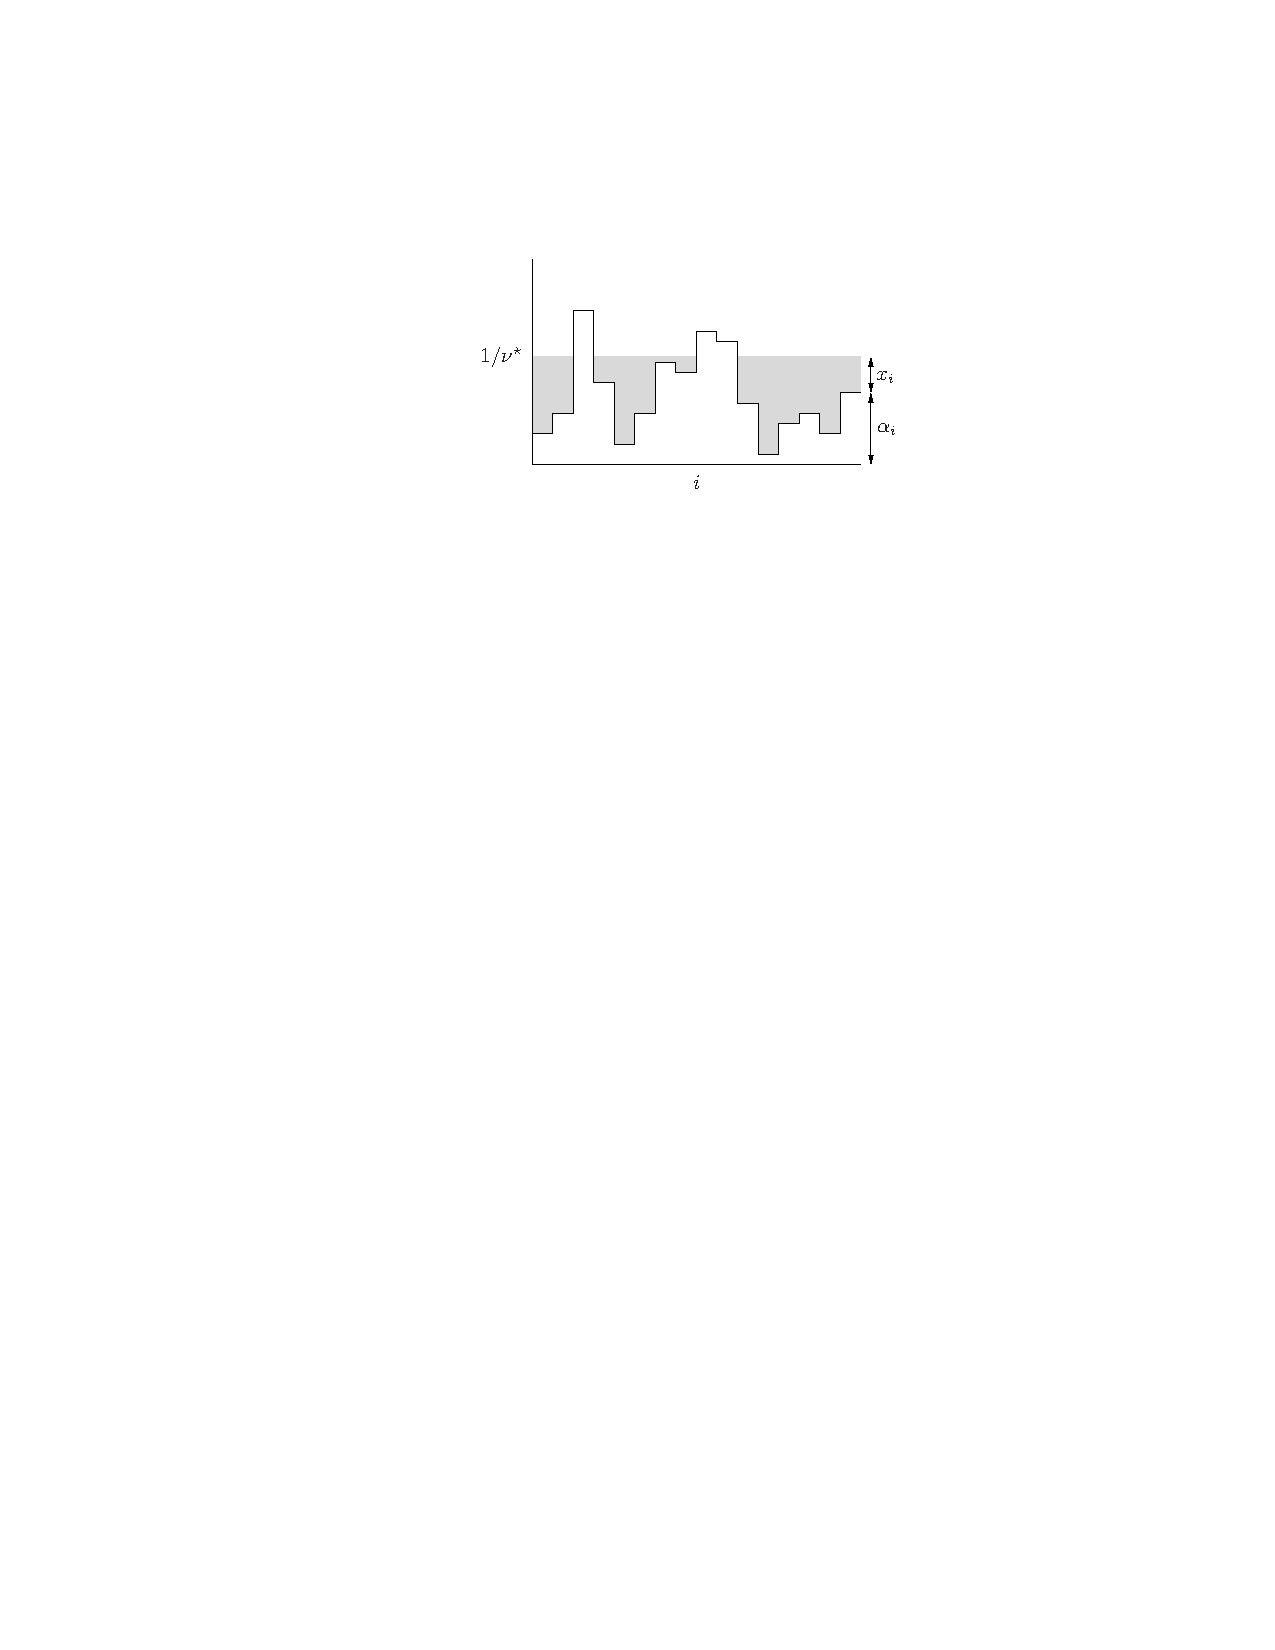
\includegraphics[width=.8\linewidth]{fig/cvbook_illu.pdf}
      \caption{Illustration of water-filling algorithm. The height of each patch is
      given by $\alpha_i$. The region is flooded to a level $1/\nu^*$ which uses a total quantity
      of water equal to one. The height of the water (shown shaded) above each
      patch is the optimal value of $x^*_i$.
      \copyright~[2022] Cambridge University Press. Reprinted, with permission from Ref. \cite{boyd2004convex}.}
      \label{fig:cvbook_illu}
    \end{figure}

    The remainder of the paper is structured as follows.
    Section~\ref{sec:alg} shows the main process of algorithm implementation of finding the water level.
    Section~\ref{sec:info} gives the basic application information of Water Filling (WF) Application.
    The random data generator module and the optimization module will be elaborated in section~\ref{sec:gen} and \ref{sec:opt} respectively.
    The conclusion will be given in section~\ref{sec:conclusion}.
    Appendix~\ref{sec:get} will give information on getting and building the application.
    Appendix~\ref{sec:doc} will present the API documentation guide. 

    \begin{figure*}[t]
      \begin{lstlisting}[morekeywords={\$}]
$ ./waterfilling -h
Usage: ./waterfilling <command> [options]

Commands:
  optimize                         solve the optimization problem
  generate                         generate random test data
  (Leave empty)                    generic use

Allowed options:

Generic options:
  -v [ --version ]                 print version string
  -h [ --help ]                    produce help message

Configuration:
  -i [ --input-data ] arg          input data file name
  -o [ --output ] arg              output file name
  -p [ --precision ] arg (=6)      optimization precision, i.e. -log10(LINEAR_PRECISION)
  -k [ --iter-max ] arg (=1000)    maximum iteration times
  --print arg (=1)                 print results on console
  --plt arg (=0)                   plot results using GNU Plot
  --plt.title arg                  plot title
  --plt.file arg                   plot file name
  --plt.c.low arg (=lemonchiffon)  plot color of the lower bar
  --plt.c.up arg (=seagreen)       plot color of the upper bar
  --plt.w arg                      plot image width
  --plt.h arg                      plot image height
  -m [ --mode ] arg (=uniform)     random data mode ('uniform' or  'normal')
  -l [ --length ] arg              length of test data set
  --min arg                        min value for uniform distribution random data generation
  --max arg                        max value for uniform distribution random data generation
  --mean arg                       mean value for normal distribution random data generation
  --sigma arg                      standard deviation for normal distribution random data generation
  --abs arg (=1)                   abs generated data
  --norm arg                       normalize generated data
  --norm-dim arg (=2)              norm dimension
      \end{lstlisting}
    \end{figure*}

  \section{Algorithm Choosing}\label{sec:alg}

    \IEEEpubidadjcol
    There can be two methods of finding the optimal water level.
    First is to sort the vector $\alpha$ and fill water level by level.
    The good point of this method is that it can yield an accurate solution.
    Another method is using the dichotomy, which is detailed in Alg.~\ref{alg}.
    The main idea is to compare the current sum of water with expected sum and then adjust the upper limit or lower limit.
    Therefore, the parameter $\varepsilon$ is needed to specify the accuracy we expect, which works together with maximum iteration counts $k$ to determine the termination of iteration update of the water level $1/\nu^*$.

    \begin{algorithm}[htbp]
      % \small
      \caption{Dichotomy Implementation of Water Filling}
      \begin{flushleft}
        \textbf{Input}: $\alpha, k, \varepsilon$.\\
        \textbf{Init}: $n=\|\alpha\|_0,(1/\nu)_{\min}=1/n,(1/\nu)_{\max}=(\|\alpha\|_1+1)/n$.
      \end{flushleft}
      \begin{algorithmic}[1]
        \For{$i=1:k$}
          \State $l=((1/\nu)_{\min}+(1/\nu)_{\max})/2$;
          \Comment Water level.
          \For{$j=0:n$}
            \State $\hat{x}_i=\max\{0,l-\alpha_i\}$;
          \EndFor
          \If{$|\|\hat{x}\|_1-1|<\varepsilon$}
            \State \textbf{break};
            \Comment Accurate enough.
          \Else
            \If{$\|\hat{x}\|_1<1$}
              \State $(1/\nu)_{\min}=l$;
              \Comment Update lower limit.
            \Else
              \State $(1/\nu)_{\max}=l$;
              \Comment Update upper limit.
            \EndIf
          \EndIf
          \EndFor
        \State $\nu^*=\nu,x=\hat{x}$;
      \end{algorithmic}
      \begin{flushleft}
        \textbf{Output}: $\nu^*$, $x$.
      \end{flushleft}
      \label{alg}
  \end{algorithm}
  Compared with the other approach,
  this method is especially efficient when the size of $\alpha$ is very large.
  
  \section{Application Information}\label{sec:info}

    The WF application is written using C++ with CMake, and has dependencies on Boost C++ Libraries and Gnuplot which will be elaborated on in Appendix~\ref{sec:get}.
    This application can work on Linux, MacOS and Windows.

    All commands and options used in the application can be found by using the option \texttt{-h} or \texttt{---help}, and the result is listed at the top of the page.    

  \section{Generating Random Data}\label{sec:gen}

  The most basic random data generation is listed below.
  The command name is \texttt{generate}, followed by options \texttt{-o} specifies the location of the generated data file and \texttt{-l} specifying the length of test data.
  \begin{lstlisting}[morekeywords={\$}]
$ ./waterfilling generate -odata.txt -l10
0.13047, 0.0612013, 0.787236, 0.655578, 0.500067, 0.684892, 0.178797, 0.651522, 0.287236, 0.0575645
  \end{lstlisting}

  Currently, WF provides two kinds of random distributions, including uniform distribution and normal distribution specified by option \texttt{-m} or \texttt{---mode}.
  Besides, you can get the absolute value by setting \texttt{--abs} to \texttt{true}. You can also normalize the data by using option \texttt{---norm} and \texttt{---norm-dim}, where the default of norm dimension is 2.

  The following example uses the normal distribution, where $\alpha_i\sim\mathcal{N}(0.5,2^2)$ and then it is normalized by 1-norm to 1.
  \begin{lstlisting}[morekeywords={\$}]
$ ./waterfilling generate -odata.txt -l10 -mnormal --mean 0.5 --sigma 2 --abs true --norm 1 --norm-dim 1
0.0422217, 0.1123, 0.00212039, 0.0480777, 0.131173, 0.231008, 0.057158, 0.160638, 0.0224425, 0.19286
  \end{lstlisting}
  The uniform distribution can implemented similarly. Here by specifying \texttt{---print} to \texttt{false}, no data will be printed on the terminal.
  \begin{lstlisting}[morekeywords={\$}]
$ ./waterfilling generate -odata.txt -l10 -muniform  --min 0 --max 1 --norm 1.5 --norm-dim 2 --print false
  \end{lstlisting}

  It should be noticed if option \texttt{-o} is not specified, the generated data will not be saved.

  \section{Optimization Implementation}\label{sec:opt}

    With data in file \texttt{data.txt}, use command \texttt{optimize} and then the result will be printed on the terminal.
    \begin{lstlisting}[morekeywords={\$}]
$ ./waterfilling optimize -idata.txt
0.394069, 0.119994, 0, 0.0157279, 0.180826, 0, 0.0189609, 0, 0.270417, 0
    \end{lstlisting}

    You can set the output file using \texttt{-o} and set \texttt{--print} to \texttt{false}.
    Precision is set using \texttt{-p} or \texttt{---precision}, max iteration is set using \texttt{-k} or \texttt{---iter-max}.

    \begin{lstlisting}[morekeywords={\$}]
$ ./waterfilling optimize -idata.txt -oresult.txt --print false -p8 -k500
    \end{lstlisting}

    To plot, make sure you have Gnuplot installed on your PC.
    You can install it on Linux or MacOS easily.
    \begin{lstlisting}[language=sh, morekeywords={\$}]
$ sudo apt-get install gnuplot # Ubuntu or Debian
$ sudo pacman -Syu gnuplot     # Arch
$ sudo port install gnuplot    # MacOS with MacPort
    \end{lstlisting}
    For Windows users, you need to add system path after installing Gnuplot.

    WF provides a wide range of image output format, including \texttt{png}, \texttt{jpg}, \texttt{jpeg}, \texttt{eps}, \texttt{pdf}, \texttt{svg}, and even \texttt{tex} TikZ plot, where the \texttt{---plt} option should be set to \texttt{true}. \texttt{---plt.file} sets the output file name and this should be distinguished from the option \texttt{---plt.title} which adds a title above the graph.
    The following example creates an eps image with the default settings.
    The $y$-axis of the image is auto scaled so it always looks good.
    \begin{lstlisting}[morekeywords={\$}]
$ ./waterfilling optimize -idata.txt --plt true --plt.file plot.eps
0.394069, 0.119994, 0, 0.0157279, 0.180826, 0, 0.0189609, 0, 0.270417, 0
    \end{lstlisting}
    The output image is shown in Fig.~\ref{fig:plot_10_eps}\footnote{All these images are generated on MacOS Big Sur (M1 chip) with Gnuplot 5.4. The generated images can be different on different platforms or with different versions of Gnuplot.}.
    \begin{figure}[htbp]
      \centering
      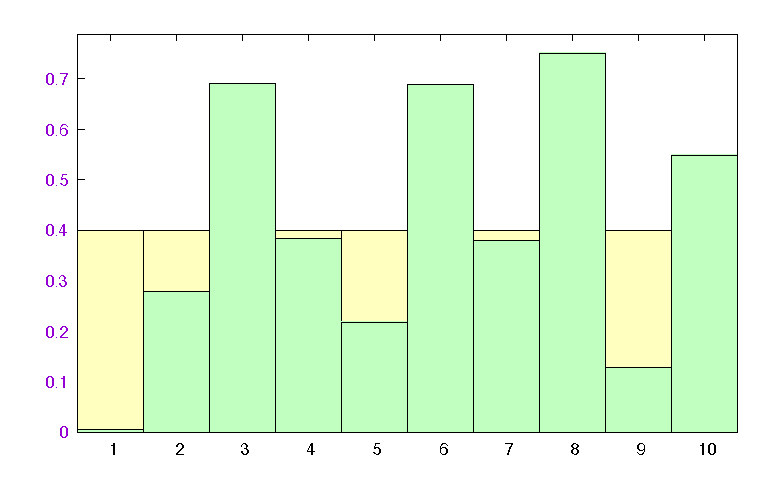
\includegraphics[width=\linewidth]{fig/plot_10.eps}
      \caption{Eps plot with the default settings.}
      \label{fig:plot_10_eps}
    \end{figure}

    You can also set its size and color with option \texttt{---plt.w} for width, \texttt{---plt.h} for height, \texttt{---plt.c.up} for upper bar color and \texttt{---plt.c.low} for lower bar color. The following example uses the TikZ plot with \texttt{tex} extension.
    Notice that the naming for colors should follow the requirements of Gnuplot.
    \begin{lstlisting}[morekeywords={\$}]
$ ./waterfilling optimize -idata.txt --print false --plt true --plt.file plot.pdf --plt.title "Water Filling Optimization Result" --plt.w 4 --plt.h 3 --plt.c.up "#dda0dd" --plt.c.low royalblue
    \end{lstlisting}
    The output image is shown in Fig.~\ref{fig:plot_10_pdf}.
    \begin{figure}[htbp]
      \centering
      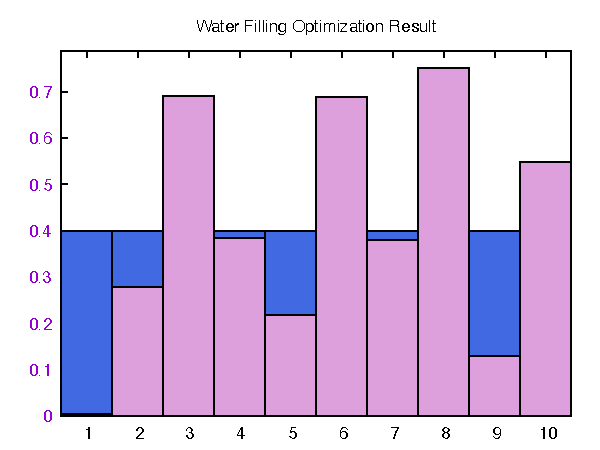
\includegraphics[width=\linewidth]{fig/plot_10.pdf}
      \caption{Pdf plot with customized settings.}
      \label{fig:plot_10_pdf}
    \end{figure}

    The WF application can deal with more data and therefore an even more magnificent image  is generated shown in Fig.~\ref{fig:plot_100_eps} with the following commands.
    \begin{lstlisting}[morekeywords={\$}]
$ ./waterfilling generate -odata.txt -l100 --norm 1.5 --print false
$ ./waterfilling optimize -idata.txt --plt true --plt.file plot.eps --plt.h 2 --plt.w 20 --print false
    \end{lstlisting}

    Most options concerning the optimization implementation has been convered and more options will be aded in the future update to make the WF application even more powerful.

    \begin{figure*}
      \centering
      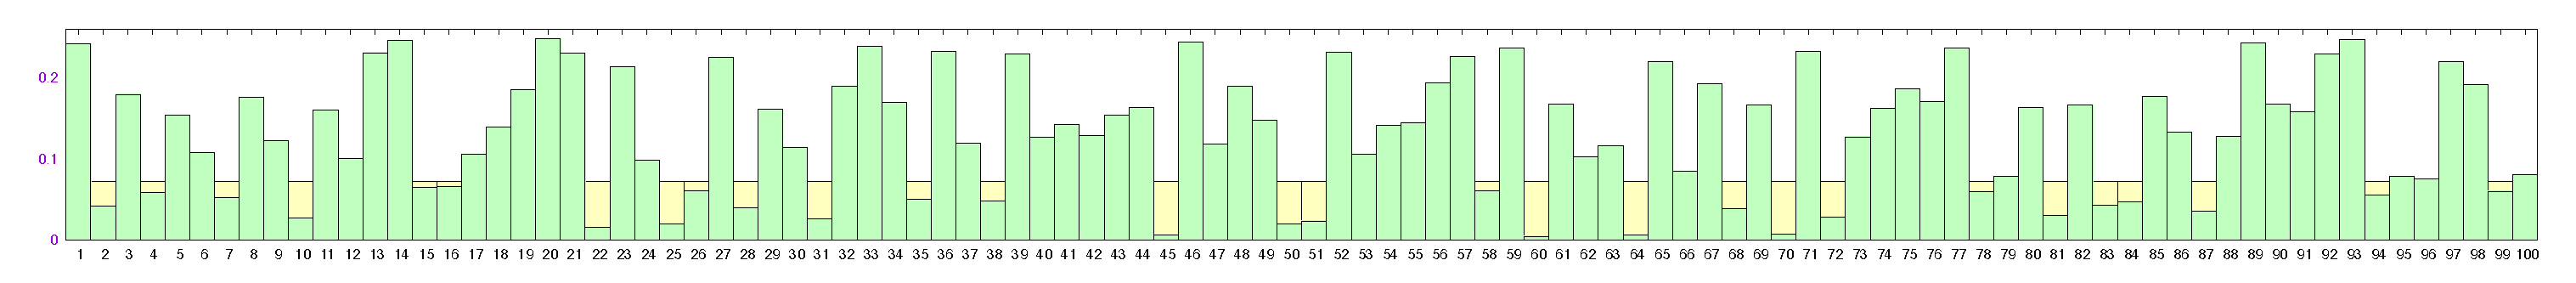
\includegraphics[width=\linewidth]{fig/plot_100.eps}
      \caption{Eps plot with generated data size of 100.}
      \label{fig:plot_100_eps}
    \end{figure*}

  \section{Conclusion}\label{sec:conclusion}

    This paper gives a brief intriductinon to the Water Filling (WF) application.
    The main contribution of the paper is that the author designs an open source application with command line interface,
    making it easy to optimize the water filling problem.
    Besides, the support of plotting adds a new dimension to the application which is now intersting to use and easy to view the optimized result.
    In the future, more options will be added to make the application to have a even wider range of use.

\appendices
  \section{Get and Build the Application}\label{sec:get}

    \begin{wrapfigure}{r}{0.32\linewidth}
    
\includegraphics[width=\linewidth]{fig/logo.eps} 
    \caption{WF Logo}
    \label{fig:logo}
    \end{wrapfigure}

    The project of WF is open source licensed under the MIT License at GitHub,
    and the repository is \href{https://github.com/Teddy-van-Jerry/Water_Filling}{Teddy-van-Jerry/Water\_Filling} \cite{web:WF}.
    You can clone or download the build binary package or source file in the release page.
    Since the build version may not be compatible with your system so it is strongly recommended that you build the project yourself with CMake which is open source available at \cite{web:cmake}.
    To compile, you need a C++ compiler supporting at least C++ 17 standard \cite{isocpp} and the Boost library available at \cite{web:boost}.
    To use the plotting function of WF, you need to have Gnuplot available at \cite{web:gnuplot}.

    With the requirements met, you can compile with the command \texttt{cmake} or to specify the Boost root directory with the command listed below.
    \begin{lstlisting}[morekeywords={\$}]
$ cmake . -DBOOST_ROOT=<dir>
    \end{lstlisting}
    If this process is successful, the executable will appear in directory \texttt{bin}.




    % \begin{figure}[htbp]
    %   \centering
    %   \subfloat{
\includegraphics[width=.3\linewidth]{fig/logo.eps}}
    %   \subfloat{
    %   \textsc{\huge Water Filling}\\A C++ Command Line App \\to optimize the water filling problem with plotting support
    %   }
    %   \caption{Water Filling logo.}
    % \end{figure}

  \section{Application Documentation}\label{sec:doc}

    WF has the API documentation generated by Doxygen at \url{https://wf.teddy-van-jerry.org}.
    The example Doxygen page is shown in Fig.~\ref{fig:doxygen}

    All classes and functions related to WF are in the namespace \texttt{wf}, which distinguishes them from dependency repository classes and functions like those of \texttt{iostream-gnuplot} open source at \cite{web:gnuplot-iostream}.
    Three main classes \texttt{WaterFilling}, \texttt{Generator} and
    \texttt{Params} work separately, making them easy to maintain.
    
    Since this project is open source, you are welcome to pull request at GitHub or publish issues.

    \begin{figure}[htbp]
      \centering
      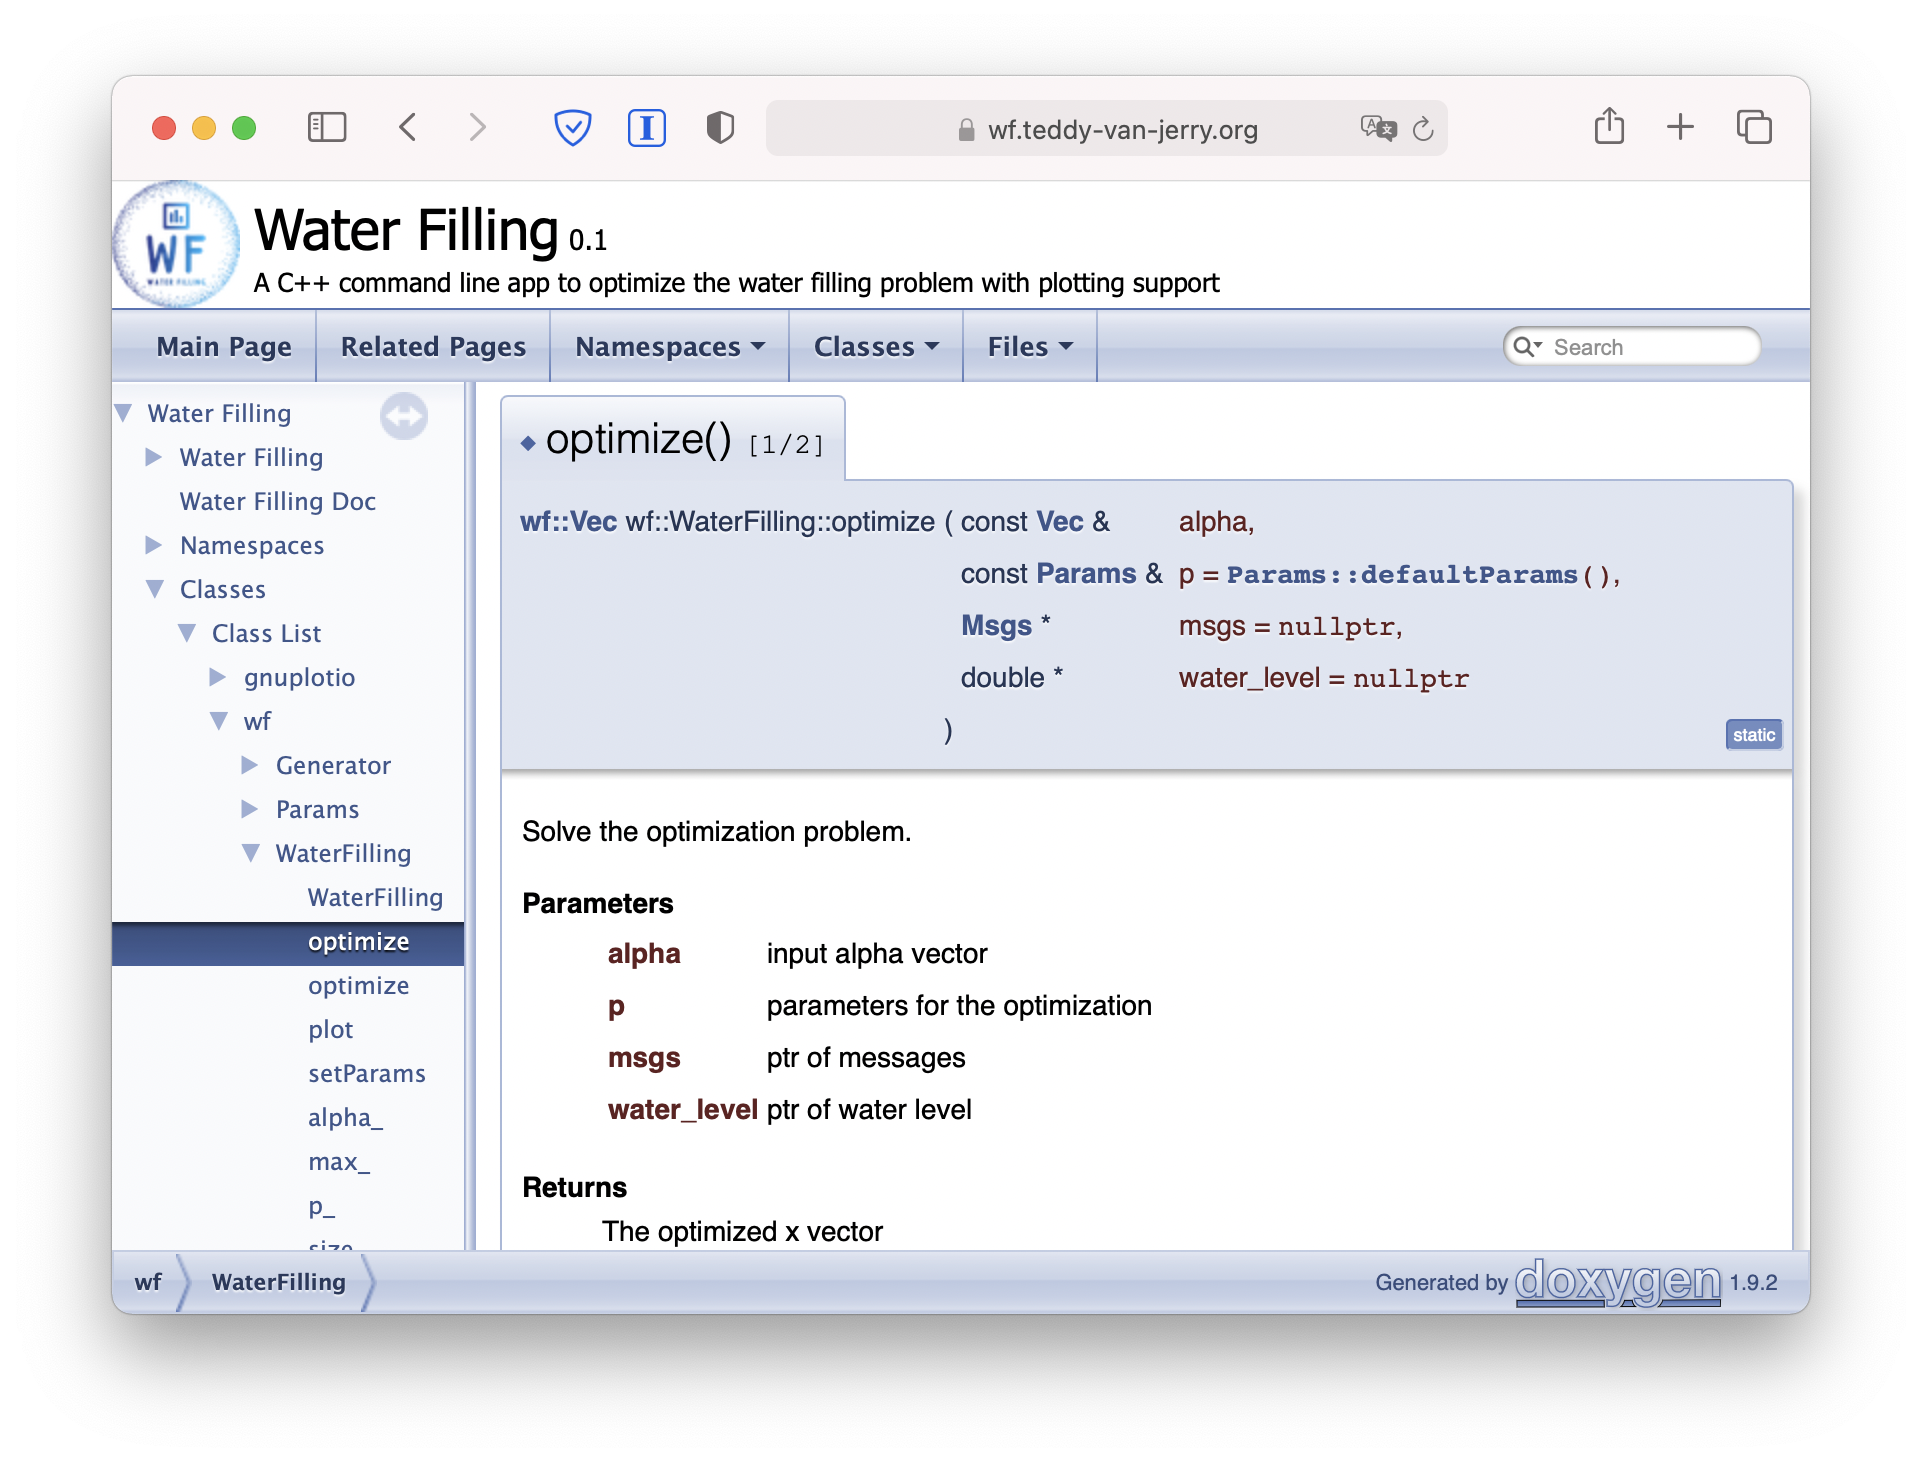
\includegraphics[width=\linewidth]{fig/doxygen.png}
      \vspace{-8mm}
      \caption{API documentation generated using Doxygen.}
      \label{fig:doxygen}
    \end{figure}

  \appendices

  

  \bibliographystyle{IEEEtran}
  \bibliography{IEEEfull, ref.bib}
  \vspace{-0.5cm}
  \begin{IEEEbiography}[{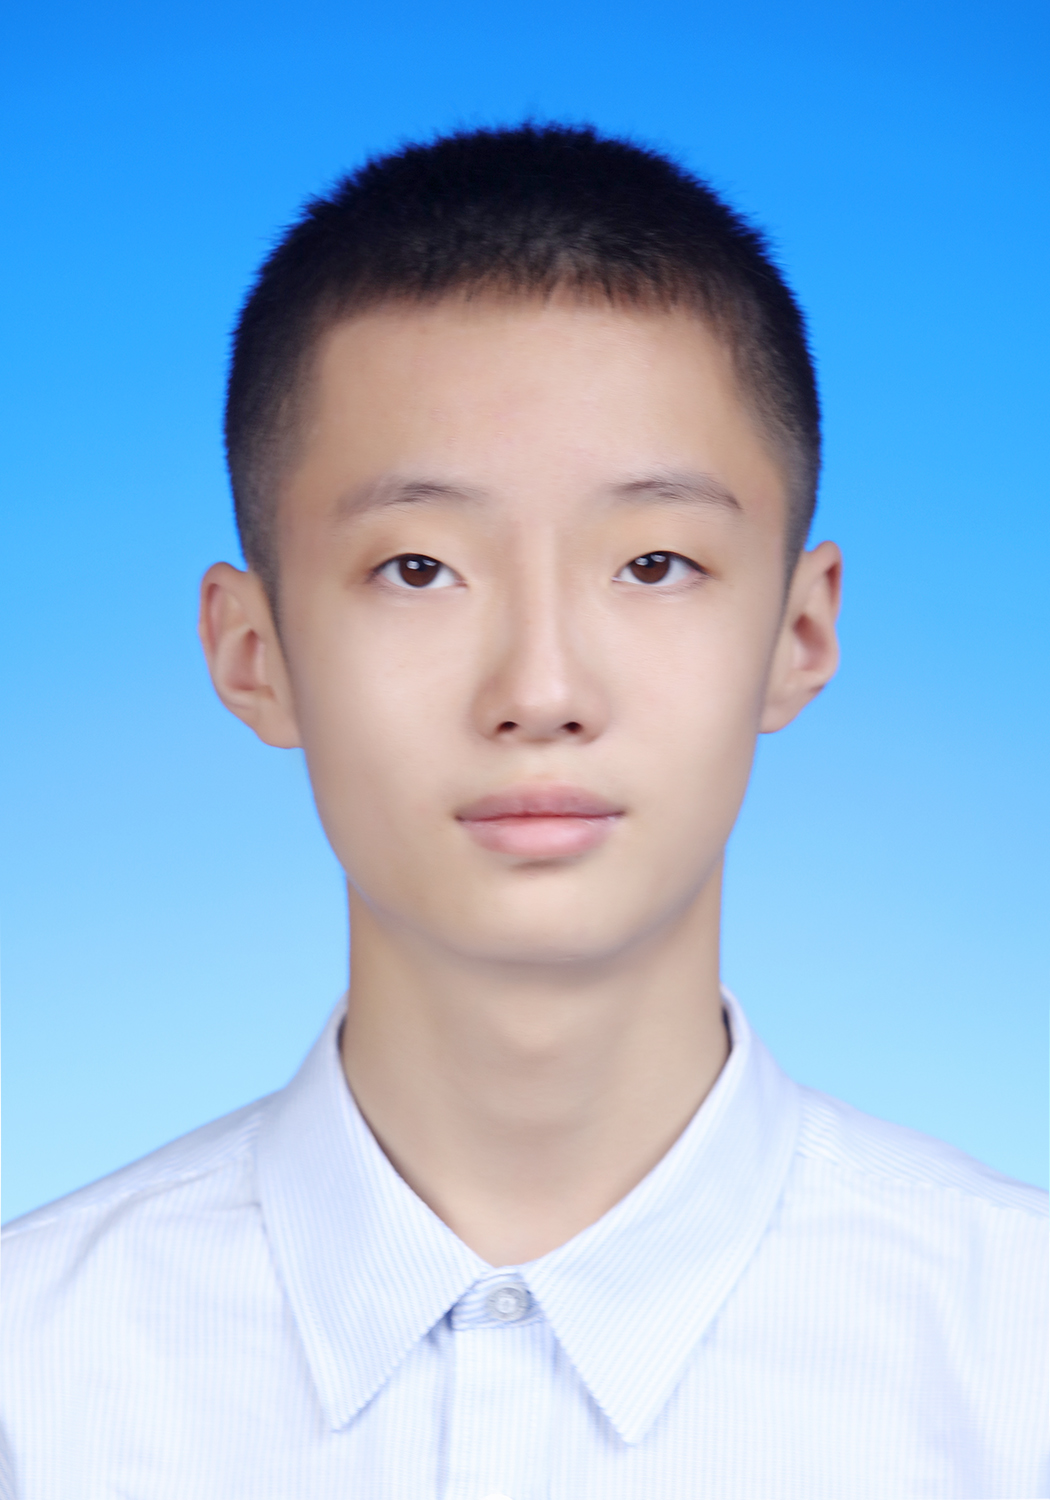
\includegraphics[width=1in,height=1.25in,clip,keepaspectratio]{fig/photo.jpg}}]%
    {Wuqiong Zhao} (Student Member, IEEE)
    is an undergraduate student pursuing the Bachelor's Degree in information science, working at Lab of Efficient Architectures for Digital-communication and Signal-processing (LEADS) and National Mobile Communications Research Laboratory, Southeast University.
    He is the honors (number one) student of Chien-Shiung Wu College which is a pilot college and training ground in Southeast University to cultivate top-notch undergraduate students selected from multiple science and engineering departments.
    He earned the National Scholarship and Cyrus Tang Scholarship in 2021.
    His research interest includes channel estimation, Bayesian algorithms, and the intelligent reflecting surface (IRS) in wireless communication of 5G and 6G.
    He assisted editing the book `Channel Codes for 5G Wireless Systems' and the chapter `Stochastic Computation for Baseband Processing'.
    He is now working on the research `OMPL-SBL Algorithm for Intelligent Reflecting Surface Channel Estimation'.
  \end{IEEEbiography}

\end{document}